\section{Encoding Total and Partial Orderings}
In the design of our encoding scheme, we assumed that the sequences to encode have no ordering: no element in a set is greater or less than any other element. In many cases, this is true, as in the example of encoding lists of next-hops, but this is not true for all applications. For the example of encoding paths of middleboxes, the middleboxes must be traversed in the order originally specified. As our scheme currently stands, this ordering is lost after the sequence is converted to a tag. 

\subsection{Total Ordering}
It is possible to impose an ordering upon the elements encoded by the tags. If the forwarding table entries which test for element membership were prioritized such that testing for element $X$ always has higher priority than testing for element $Y$, then this imposes the ordering $X > Y$ on the pair. Forwarding tables return the highest priority match, so if both $X$ and $Y$ are present in the sequence, then the test for $X$ will be the test that returns true. We can use this idea to support element ordering, so long as the element set is \textit{totally ordered}.

\subsection{Partial Ordering}
It may not always be the case that the elements have a total ordering, but it may be nearly the case for some applications. If, across all sequences, there are a few pairs of elements $X$ and $Y$ such that $X$ appears before $Y$ in some sequences and $Y$ appears before $X$ in others, then $X$ and $Y$ are incomparable and we say that the universe is \textit{partially ordered}. It is still possible to encode such a list of sequences using our scheme, but at the cost of slightly larger tags.

Support for partial orderings is possible with one key observation: for a sequence to be ordered, switches must be able to perform ordered membership testing. If we have elements $[X,Y,Z]$ with $X > Y > Z$, then membership of $X$ is tested first by checking for for the $X$ bit, then $Y$, and finally $Z$. If however, we had to encode the two paths $XYZ$ and $YXZ$, this approach fails when each element is mapped to only one bit. Were we to map $X$ to two bits, one before $Y$ and one after $Y$, then $XYZ$ could be encoded as $1101$ and $YXZ$ would be $0111$. The bits could be tested in order from left to right, and both paths would be recreated correctly. 

To convert from a partial ordering to a totally ordered sequence of bits, incomparable pairs of elements could be made comparable by \textit{splitting} of one of the bits. For example, consider an incomparable pair $(B, C)$. We could split $B$ into bits $B_1$ and $B_2$. In every order where $B$ appears before $C$, we would replace $B$ with $B_1$. When $B$ appears after $C$, we would use $B_2$. This creates the ordering $B_1 < C < B_2$, resolving the incomparability! If every pair of incomparable elements is resolved with splitting, then the partially ordered universe of elements is replaced by a totally ordered new, larger universe of elements, where each element in the new universe can be mapped to an element in the original universe. We can then use this new universe to create tags for each sequence. 

\subsection{Partial to Total Ordering}

Unfortunately, converting a partially ordered universe to a totally ordered universe is not straightforward. There can potentially be sets of incomparable elements, rather than just pairs, making it unclear which elements to split to resolve incomparabilities with the least number of additional bits. In the worst case where every pair of elements is incomparable, 

 Figure \ref{fig:ordering} shows one algorithm for doing so at a high level. For a concrete example, we are given four input sequences we wish to encode, shown in \ref{fig:ordering}(a). We assume that these sequences \textit{almost} follow an underlying ordering, but that there are a few incomparable sets of elements. In this example, $B$ is incomparable with $C$ because $B$ appears both before and after $C$. 

To systematically identify these incomparable elements, we construct the sequence graph, shown in \ref{fig:ordering}(b). In the sequence graph, element $u$'s node has an edge to element $v$'s node if $u$ appears before $v$ in any sequence. We then run an algorithm for finding Strongly Connected Components (SCCs) on this graph. A strongly connected component is a set of nodes such that for every pair of nodes $u$ and $v$ in the set, $u$ has a path to $v$ and vice versa. In this context, every SCC corresponds to a set of incomparable elements. Figure \ref{fig:conflict_res} shows the process for determining which elements to split to create a new, totally ordered universe. Figure \ref{fig:ordering}(d) and (e) shows the result of using this new ordering to modify each sequence. 


\begin{figure}[t!] 
\begin{minipage}{1\linewidth}
\begin{subfigure}[c]{0.96\linewidth}
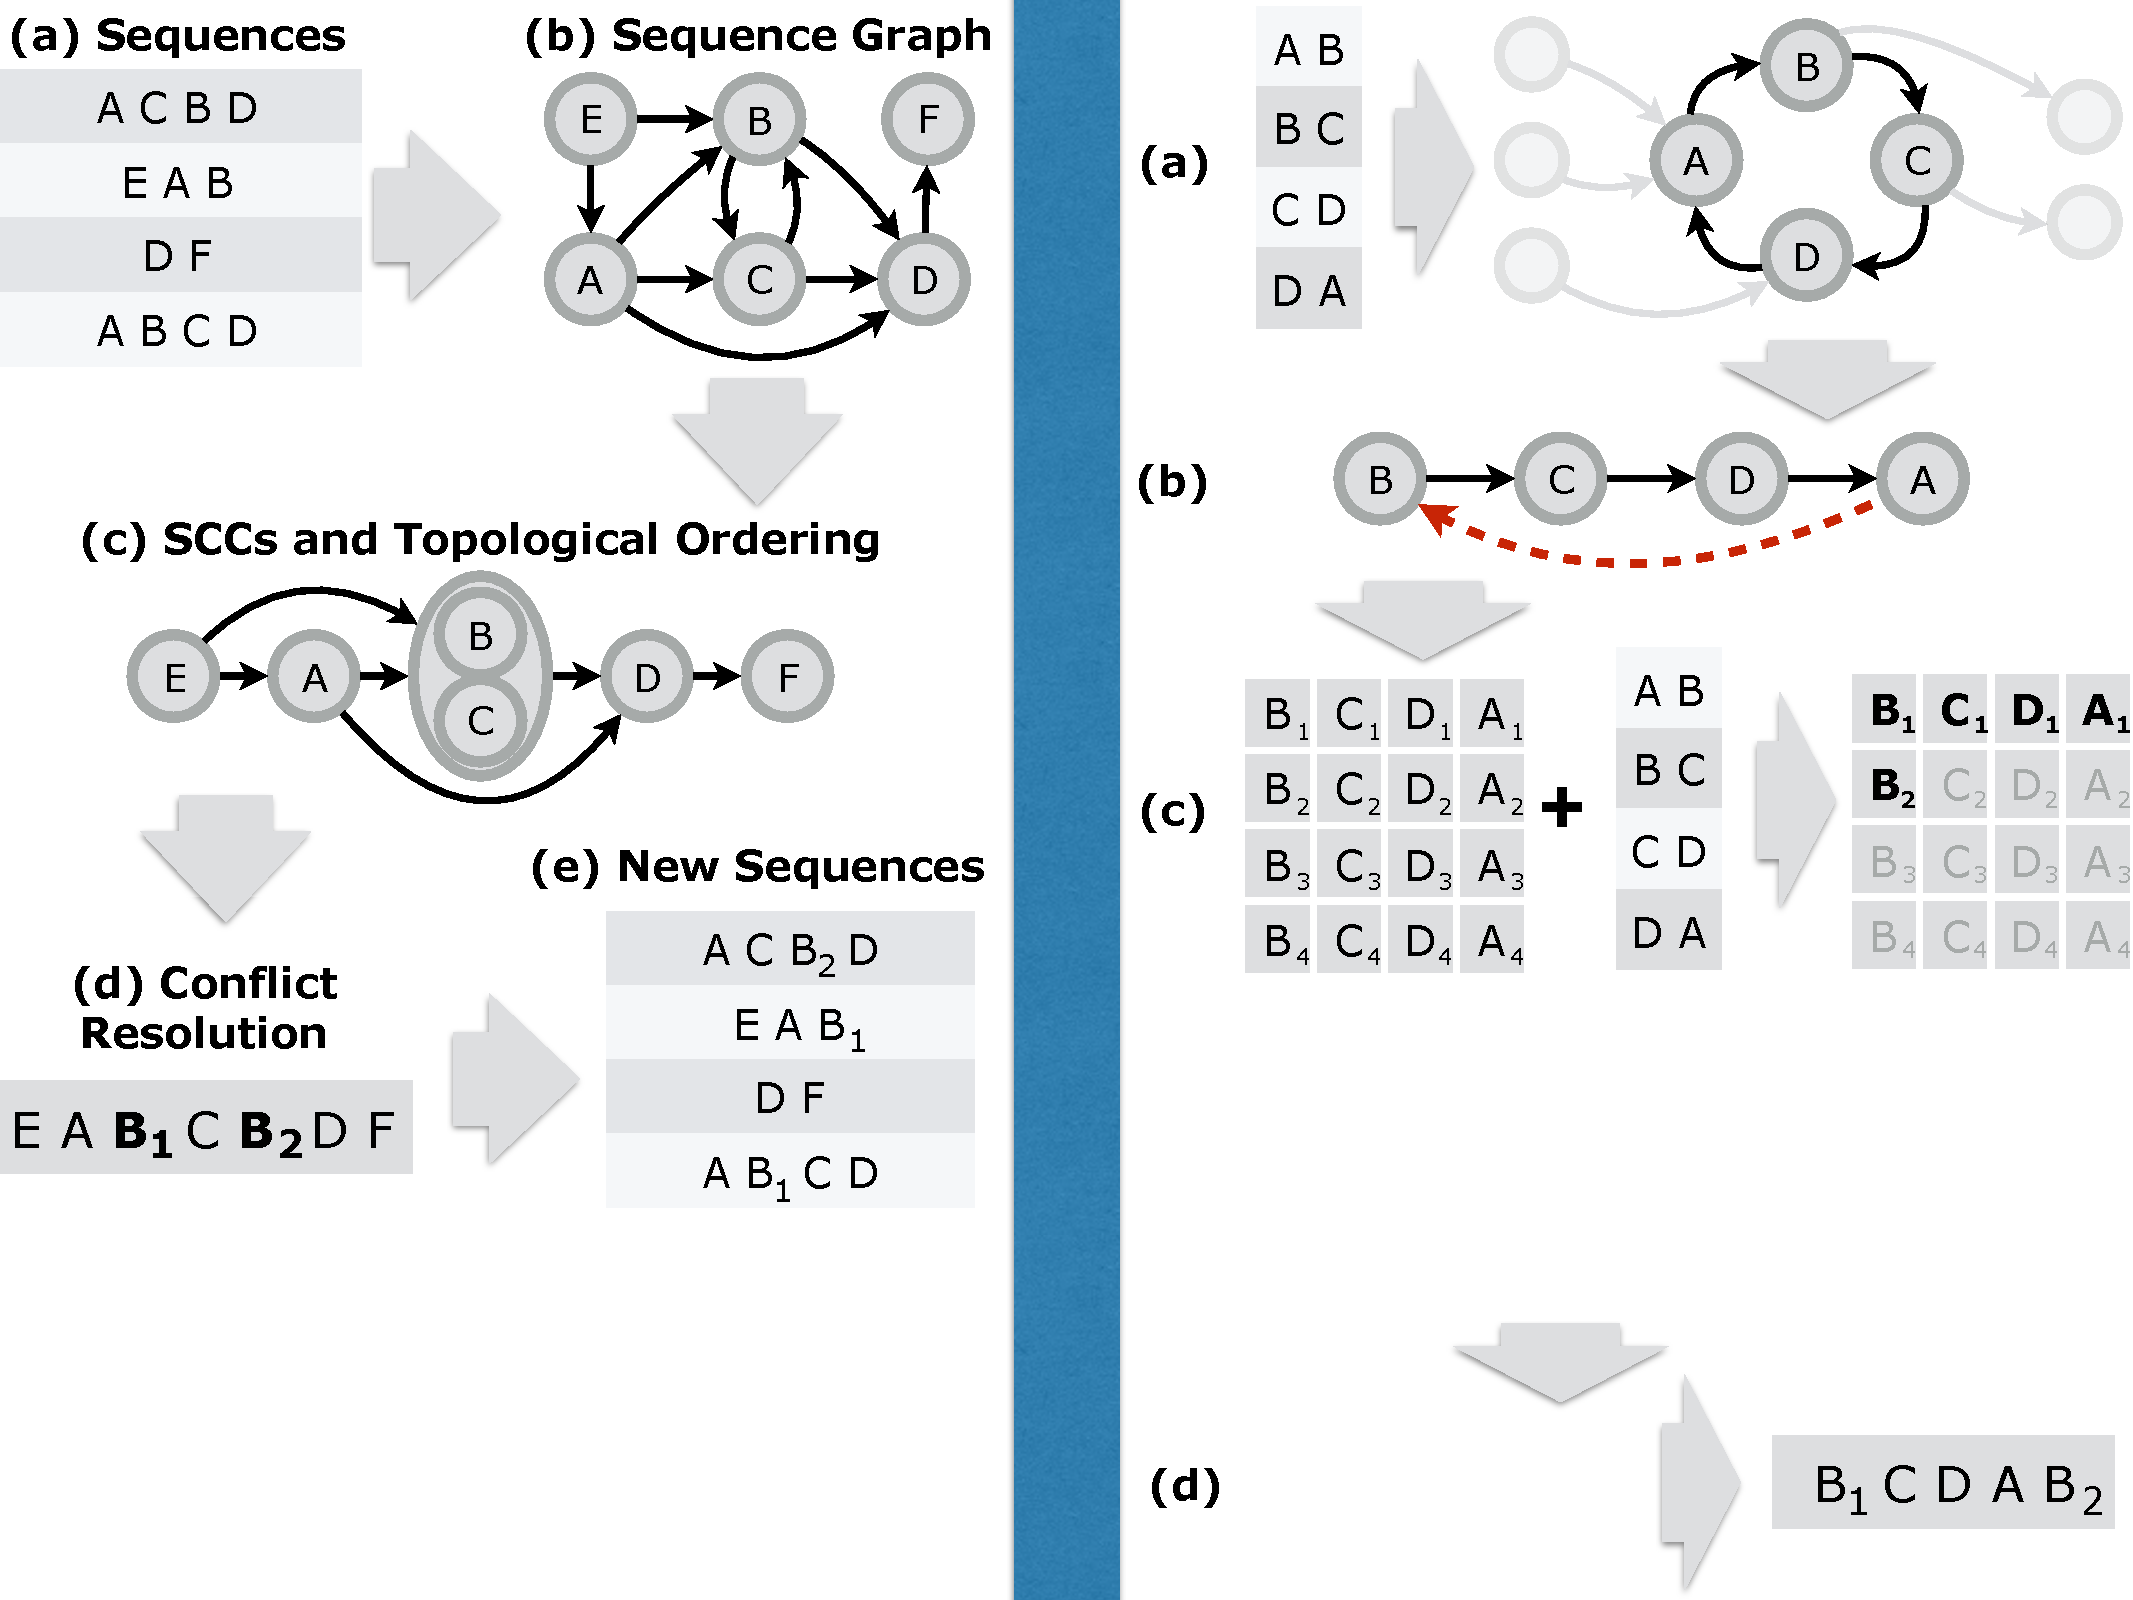
\includegraphics[trim={0 6cm 19.2cm 0}, clip, width=\linewidth]{figures/partial_ordering}
\end{subfigure} 
\end{minipage} 
\caption{This figure shows, at a high level, the process for converting a partial ordering to a total ordering by identifying incomparable elements and creating duplicates to resolve the incomparabilities. (a) shows the four input ordered sequences. In (b), we create a graph of the elements, where there is an edge from $u$ to $v$ if $u$ appears before $v$ in some sequence. (b) shows how the graph can be broken up into an ordered Directed Acyclic Graph (DAG) of Strongly Connected Components (SCC), where each SCC corresponds to a set of incomparable elements. (d) shows the result of splitting elements to resolve incomparability, which is covered in more depth in figure \ref{fig:conflict_res}. In (e), the original sequences are modified with the splits such that each sequence adheres to a total ordering.}
\label{fig:ordering}
\end{figure}



\begin{figure}[t!] 
\begin{minipage}{1\linewidth}
\begin{subfigure}[c]{0.96\linewidth}
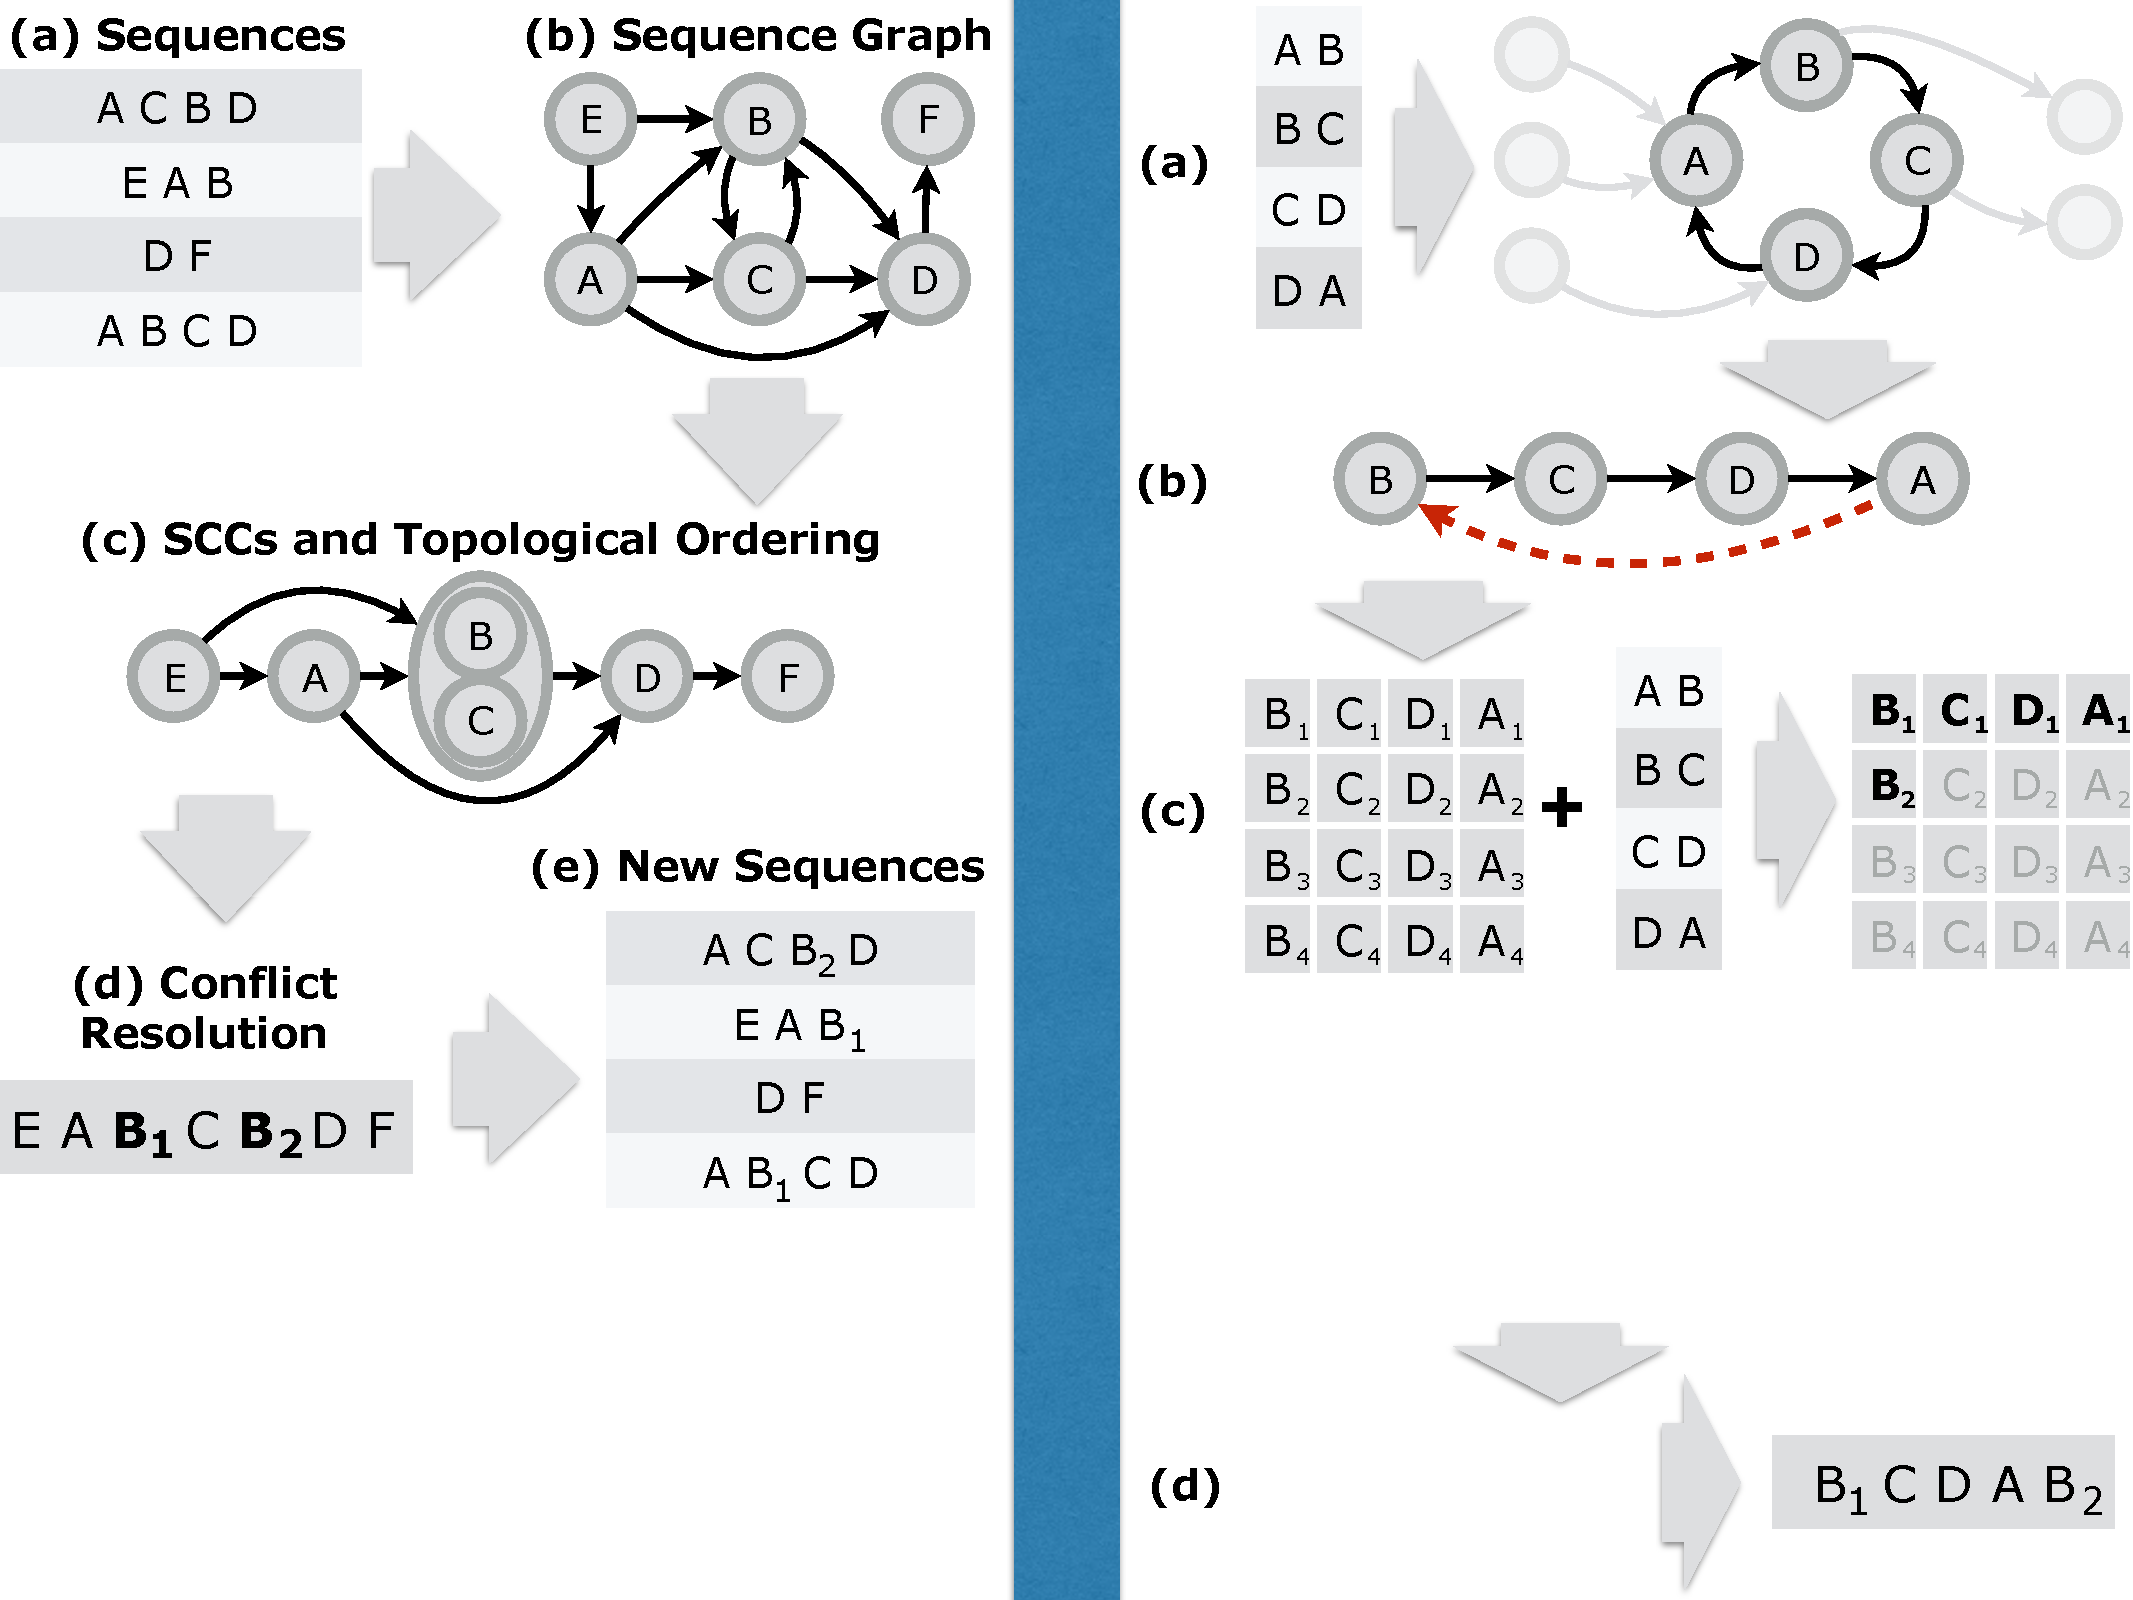
\includegraphics[trim={19.2cm 10cm 0 0}, clip, width=\linewidth]{figures/partial_ordering}
\end{subfigure} 
\end{minipage} 
\caption{This details the Conflict Resolution step of the algorithm. (a) shows a SCC corresponding to four incomparable elements. (b) shows an 'almost' ordering of the SCC nodes, which minimizes the number of backward edges. (c) shows how the almost ordering is used to construct a worst-case quadratically-sized universe, which is then traversed by every sequence to determine which splits are necessary. }
\label{fig:conflict_res}
\end{figure}